\chapter{Foutafhandeling}

\begin{summary}
Tijdens het uitvoeren van een programma kan en zal er vanalles foutgaan. De gebruiker van het programma geeft de datum in in een foutief formaat, een printer is offline, er is onvoldoende schrijfruimte vrij om een bestand weg te schrijven, het programma kreeg onvoldoende geheugen toegewezen,... Fouten die zich voordoen tijdens het uitvoeren van een programma, at runtime dus, verdelen we onder in errors en exceptions. Errors zijn de fouten die meestal veroorzaakt worden door het onderliggende besturingssysteem. Tijdens het verloop van het programma kunnen deze errors niet meer opgelost worden en het programma zal daarom be\"eindigd worden. Dit is niet het geval voor exceptions. Je kan je code op een defensieve manier schrijven en rekening houden met de mogelijke exceptions die kunnen optreden. ``Exception handling'' is het proces om deze exceptions op een correcte en liefst gebruiksvriendelijke manier af te handelen. Indien een fout niet correct wordt afgehandeld, zal het programma alsnog voortijdig afgebroken worden, maar met de juiste foutafhandeling kan de uitvoer van het programma gewoon verdergezet worden. 
 \end{summary}
 
\section{Compile-time vs runtime errors}

Een programmeur schrijft Java code in zijn editor of favoriete IDE. Vervolgens wordt de Java code gecompileerd tot bytecode. Deze bytecode wordt door de JVM (Java Virtual Machine) ge\"interpreteerd tot machinecode instructies die worden uitgevoerd door het computersysteem.

Wanneer dus een Java programma wordt opgestart, kunnen er 2 categorie\"en van problemen voorkomen. Het kan zijn dat het Java programma niet gecompileerd kan worden. In dat geval spreken we van een compile-time error. Indien het programma succesvol gecompileerd wordt, kan er zich tijdens het uitvoeren van de code een probleem voordoen, in dat geval spreken we van runtime errors of exceptions. 

\begin{figure}[H]
  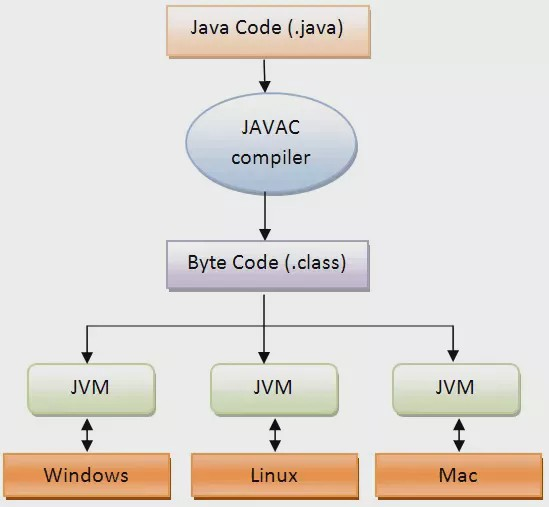
\includegraphics[width=\linewidth]{images/h1/java_compiler.jpeg}
  \caption{Compiler, interpreter en Java Virtual Machine.}
  \label{fig:compiler}
\end{figure}


\begin{figure}[H]
  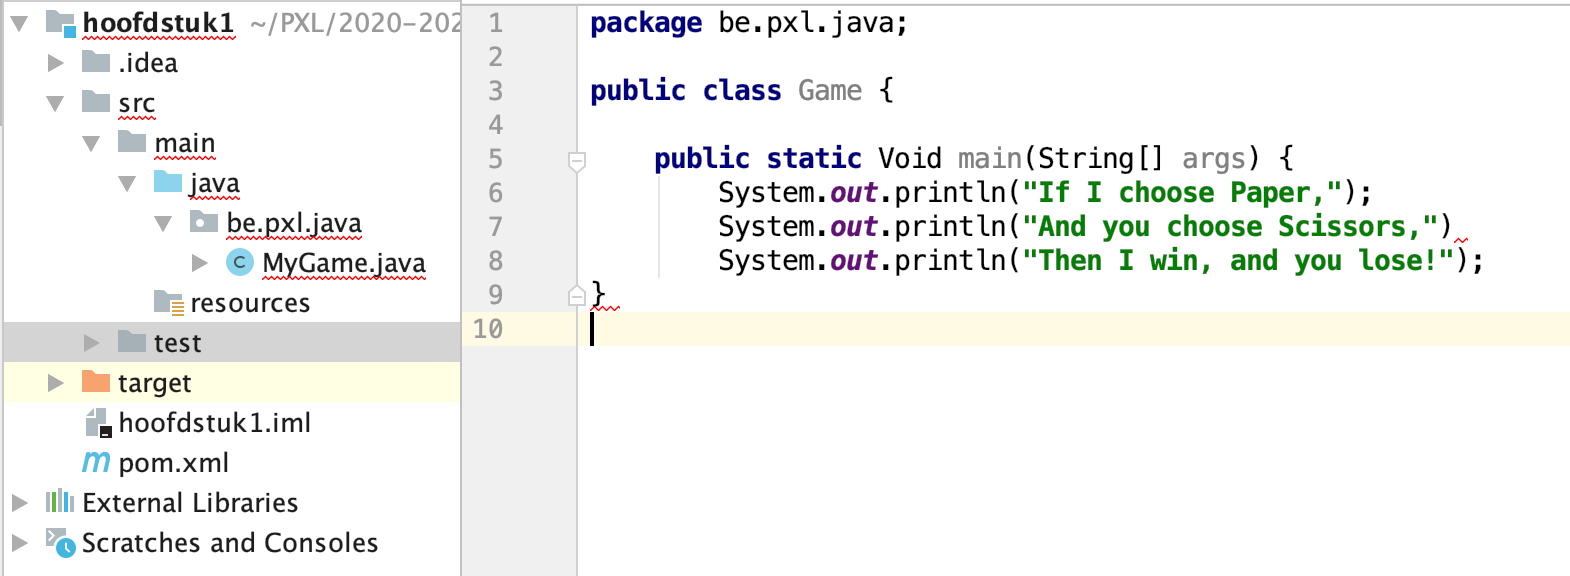
\includegraphics[width=\linewidth]{images/h1/compiletime_errors.png}
  \caption{Compile-time errors}
  \label{fig:compiletime_errors}
\end{figure}

\begin{oefening}
Welke compile-time errors kan je ontdekken in het volgende codefragment in figuur \ref{fig:compiletime_errors}?
\end{oefening}

Omdat Java een object-ge\"orienteerde programmeertaal is, wordt er ook een object gebruikt om aan te geven dat er iets fout ging bij uitvoeren van het Java programma. Zodra er zich een probleem voordoet tijdens het uitvoeren van een programma-instructie, wordt er een exception-object aangemaakt en ``opgeworpen''. Hierdoor stopt de normale uitvoer van het programma. Er wordt nog geprobeerd om het exception-object op een keurige manier af te handelen (indien die code aanwezig is), maar als dat niet lukt zal het programma be\"eindigd worden. Het exception-object bevat nuttige informatie voor de ontwikkelaar zoals de methode en lijn-nummer waar de exception werd aangemaakt en het type van de exception. 

\section{First catch}

\begin{lstlisting}
public class DivisionByZero {

	public static void main(String[] args) {
		int a = (1 + 1) % 2;
		int b = 5;
		int c = b / a;
		System.out.println("Het resultaat is " + c);
	}
}
\end{lstlisting}

Als je het bovenstaande programma uitvoert zal het volgende in de console verschijnen:

\begin{verbatim}
Exception in thread "main" java.lang.ArithmeticException: / by zero
	at be.pxl.ja.DivisionByZero.main(DivisionByZero.java:6)<5 internal calls>
\end{verbatim}
  
De variabele \textit{a} bevat inderdaad de waarde 0 en hierdoor hebben we dus te maken met een deling door 0. Zodra de deling wordt uitgevoerd loopt het dus fout en gooit de java runtime een ArithmeticException op. Omdat de ArithmeticException nergens wordt afgehandeld eindigt het programma. Je zal enkel nog een stacktrace zien verschijnen in de console. Een stacktrace is de naam en foutboodschap van de exception gevolgd door de weg die de exception heeft afgelegd (doorheen de methoden van je klassen) vanaf het moment dat ze werd opgegooid. We zien dus dat de exception is veroorzaakt op regel 6 in de klasse DivisionByZero.

\begin{lstlisting}
public class DivisionByZero {

	public static void main(String[] args) {
		int a = (1 + 1) % 2;
		int b = 5;
		try {
			int c = b / a;
			System.out.println("Het resultaat is " + c);
		} catch (ArithmeticException e) {
			System.out.println("You should not divide a number by zero.");
		}
		System.out.println("First catch completed!");
	}
}
\end{lstlisting}

\begin{verbatim}
You should not divide a number by zero.
First catch completed!
\end{verbatim}

We hebben de instructie met de deling nu in een try-blok geplaatst. Omdat de variabele c in het try-blok wordt aangemaakt, kan deze variabele ook enkel binnen het try-blok gebruikt worden. Indien een exception optreedt binnen een try-blok zal de programma-uitvoer de resterende code binnen het try-blok overslaan en verdergaan bij het eerste catch-blok dat direct volgt achter het try-blok. Je bent als programmeur verplicht om een try-blok steeds te laten volgen door \'e\'en of meerdere catch-blokken.
In het catch-blok wordt dan de code uitgevoerd om het probleem op te lossen of tenminste een duidelijke boodschap voor de gebruiker van het programma te voorzien.
Als alle instructies uit het catch-blok zijn uitgevoerd zal het programma zijn normale uitvoer verderzetten.


\section{Java exception hi\"erarchie}
  
\begin{figure}[H]
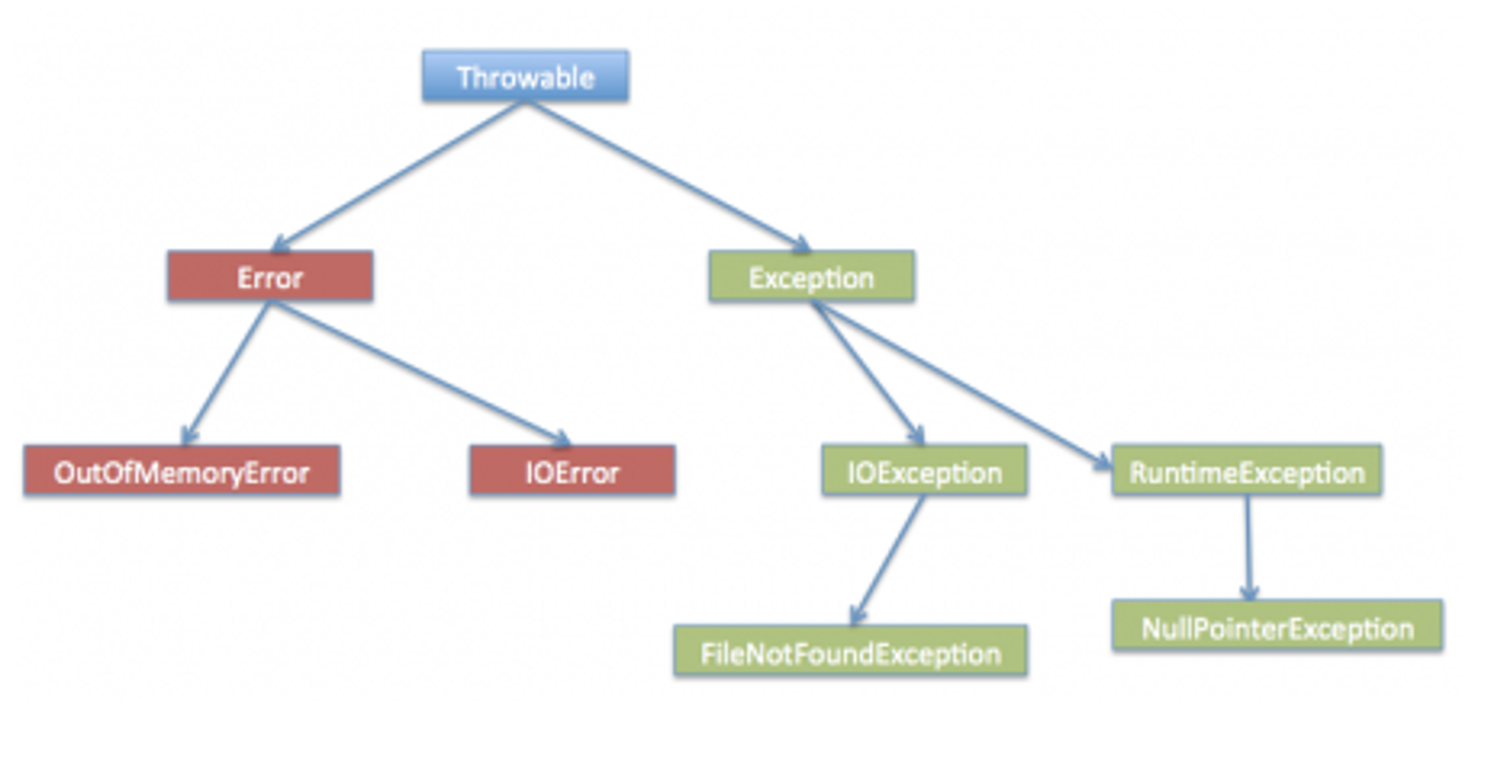
\includegraphics[width=\linewidth]{images/h1/exception-hierarchy.png}
\caption{Exception hi\"erarchie}
\label{fig:exceptiono_hierarchy}
\end{figure}
  
Zoals reeds vermeld wordt er een exception-object aangemaakt zodra zich een probleem voordoet in de code. 
Er is in Java een hi\"erarchie gebouwd van exception-klassen om verschillende soorten fouten in een programma te categorizeren. Throwable is de superklasse van alle exceptions en errors in Java. Er zijn dus 2 afgeleide klassen van Throwable: Error and Exception. Exceptions zijn nog verder onderverdeeld in \textbf{checked exceptions} en \textbf{runtime exceptions}.

\subsection{Errors}

Errors zijn problemen die zich voordoen tijdens het uitvoeren van het programma en die meestal niet gerelateerd zijn aan het programma zelf. Daarom is het onmogelijk om erop te anticiperen en te herstellen van deze fouten. Dit kan gaan van hardware falen, over JVM crashes en out of memory errors. We hebben een aparte hi\"erarchie van errors en we zullen nooit code toevoegen in ons programma om deze fouten af te handelen. We tonen hier enkel voorbeelden van errors.


\subsubsection{StackOverflowError}
Je hebt ongetwijfeld al eens per ongeluk een programma geschreven met een oneindige lus. 

\begin{lstlisting}
public class DemoStackOverflow {

	private static void printNumber(int x) {
		System.out.println(x);
		printNumber(x + 2);
	}

	public static void main(String[] args) {
		printNumber(15);
	}
}
\end{lstlisting}

\begin{verbatim}
15
17
19
...
36597
36599
Exception in thread "main" java.lang.StackOverflowError
	...
	at be.pxl.ja.DemoStackOverflow.printNumber(DemoStackOverflow.java:5)
	at be.pxl.ja.DemoStackOverflow.printNumber(DemoStackOverflow.java:5) 
	at be.pxl.ja.DemoStackOverflow.printNumber(DemoStackOverflow.java:5) 
	at be.pxl.ja.DemoStackOverflow.printNumber(DemoStackOverflow.java:5) 
	...
\end{verbatim}

De call stack is de manier waarop tijdens de uitvoer van een programma o.a. wordt bijgehouden welke functies worden aangeroepen. Wanneer je programma-uitvoer in een oneindige lus terechtkomt, stapelen de gegevens in de call stack zich razendsnel op en loopt de call stack vol. Het programma zal uiteindelijk eindigen met een StackOverflowError.

\begin{figure}[H]
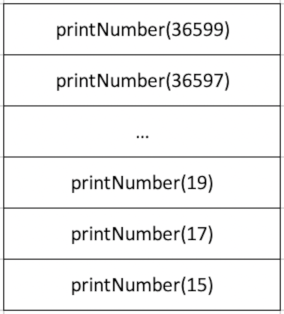
\includegraphics{images/h2/java_call_stack.png}
\caption{Java call stack}
\label{fig:call_stack}
\end{figure}


\subsubsection{OutOfMemoryError}

\begin{lstlisting}
package be.pxl.ja;

public class DemoOutOfMemory {

	private void generateOutOfMemory() {
		Long maxMemory = Runtime.getRuntime().maxMemory();
		System.out.println(maxMemory);

		int[] matrix = new int[(int) (maxMemory + 1)];
		for (int i = 0; i < matrix.length; ++i) {
			matrix[i] = i + 1;
		}
		System.out.println("Matrix filled" + matrix[(int)(Math.random() * 100)]);

	}

	public static void main(String[] args) {
		DemoOutOfMemory doom = new DemoOutOfMemory();
		doom.generateOutOfMemory();
	}
}
\end{lstlisting}

Om de OutOfMemoryError te illustreren maken we een array aan die meer geheugenplaatsen inneemt dan de ruimte die het java programma ter beschikking heeft.

Als je dit programma uitvoert, pas je best het beschikbare geheugen voor het programma aan. Dit doe je door een waarde voor de VM optie -Xmx mee te geven.

\begin{itemize}
\item -Xmssize: Geeft de initi\"ele waarde voor de heap size.
\item -Xmxsize: Geeft de maximale waarde voor heap size.
\end{itemize}

De heap size van een Java programma is de hoeveelheid geheugen dat een Java-programma mag gebruiken om objecten op te slaan.

\begin{verbatim}
67108864
Exception in thread "main" java.lang.OutOfMemoryError: Java heap space
	at be.pxl.ja.DemoOutOfMemory.generateOutOfMemory(DemoOutOfMemory.java:8)
	at be.pxl.ja.DemoOutOfMemory.main(DemoOutOfMemory.java:16)<5 internal calls>
\end{verbatim}
	
\begin{figure}[H]
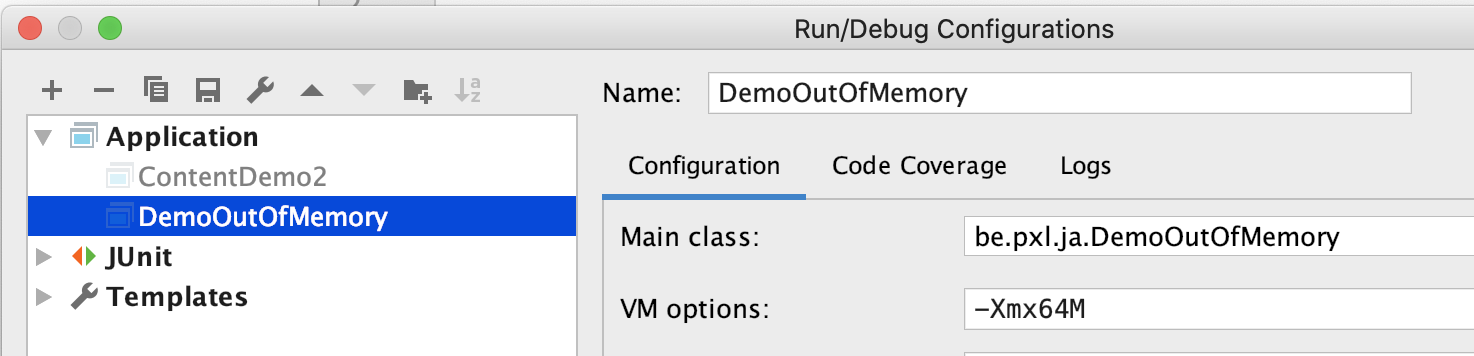
\includegraphics[width=\linewidth]{images/h2/jvm_options_xmx.png}
\caption{Maximum heap size aanpassen}
\label{fig:exceptiono_hierarchy}
\end{figure}

\subsection{Runtime exceptions}

Runtime exceptions zijn exceptions die vaak veroorzaakt worden door logische fouten in het programma.Typische voorbeelden van runtime exceptions zijn ArrayIndexOutOfBoundsException, NullPointerException en IllegalArgumentException. Vaak moet je ze niet afhandelen, maar moet je ervoor zorgen dat je de bug in je code oplost. Ook hier zijn onze unit testen heel belangrijk. Door goede unit testen te schrijven ga je runtime exceptions in je code opmerken en kunnen oplossen.

\begin{lstlisting}
package be.pxl.ja;

public class Demo {

	public static void main(String[] args) {
		String tekst = "abc";
		System.out.println(tekst.repeat(-5));
	}
}
\end{lstlisting}

\begin{verbatim}
Exception in thread "main" java.lang.IllegalArgumentException: count is negative: -5
	at java.base/java.lang.String.repeat(String.java:3586)
	at be.pxl.ja.Demo.main(Demo.java:5)
\end{verbatim}

\begin{oefening}

\begin{lstlisting}
@Service
public class MusicPlaylistService {

	private List<Song> playlist;

	public void addSong(Song song) {
		playlist.add(song);
	}
}
\end{lstlisting}

Welke exception doet zich voor zodra je de methode addSong() aanroept? Waarom treedt die exception op?
\end{oefening}

Wanneer je programma gebruikmaakt van gegevens die door de gebruiker worden ingevoerd, moet je er altijd rekening mee houden dat de gebruiker foutieve gegevens kan ingeven. Deze foutieve gegevens kunnen aanleiding geven tot runtime exceptions. Ook hier moet je steeds anticiperen op de mogelijke input die de gebruiker kan invoeren. 


\begin{lstlisting}
package be.pxl.ja;

public class ElementInArray {

	public static void main(String[] args) {
		String[] elements = { "H", "He", "Li", "Be", "B", "C", "N", "O", "F", "Ne" };

		Scanner scanner = new Scanner(System.in);
		
		// OPLOSSING 1
		System.out.println("Kies een nummer: ");
		int chosen = scanner.nextInt();
		if (chosen < elements.length) {
			System.out.println(elements[chosen]);
		} else {
			System.out.println("U koos een verkeerd nummer.");
		}

	    // OPLOSSING 2
		System.out.println("Kies een nummer: ");
		chosen = scanner.nextInt();
		try {
			System.out.println(elements[chosen]);
		} catch (ArrayIndexOutOfBoundsException e) {
			System.out.println("U koos een verkeerd nummer.");
		}
	}
}
\end{lstlisting}

In bovenstaand codevoorbeeld gaat onze voorkeur uit naar oplossing 1 waarbij de ingevoerde waarde wordt gecontroleerd vooraleer het element uit de array wordt benaderd. Deze code is makkelijker leesbaar en onderhoudbaar.


\subsection{Checked exceptions}

Wanneer je in java een methode aanroept, kan het voorkomen dat je direct een compileerfout voorgeschoteld krijgt. Het kan namelijk zijn dat java reeds anticipeert op mogelijke problemen en je dwingt om rekening te houden met het scenario dat er iets mis kan gaan. De compileerfout raakt pas opgelost wanneer je het afhandelen van de exception netjes programmeert.

Kijk eens naar onderstaand voorbeeld uit de streaming service.
We gebruiken hier de klasse MessageDigest uit JDK. Message digests zijn functies waarmee we voor input-data van willekeurige lengte een hash-waarde met een vaste lengte kunnen berekenen.  Als je de hash-waarde kent, kan je hieruit de input-data niet afleiden. We gebruiken dit om een paswoord bij te houden in een Account-object. We willen absoluut vermijden dat paswoorden in een leesbaar formaat in onze objecten worden bijgehouden.

Om een message digest te berekenen in Java moet je eerst de static methode getInstance() aanroepen met als parameter het door jouw gekozen algoritme. In dit voorbeeld wordt er gekozen voor MD5. Je ziet dat de lijn code, ondanks het feit dat alles correct is geschreven, toch rood wordt onderlijnd. Dat komt omdat de methode getInstance() een exception kan opgooien die we verplicht moeten afhandelen.

\begin{oefening}
Open de documentatie van de klasse MessageDigest en bekijk de uitleg voor de static methode getInstance(). Kan je hier zien welke exceptions er kunnen voorkomen?
\end{oefening}

\begin{figure}[H]
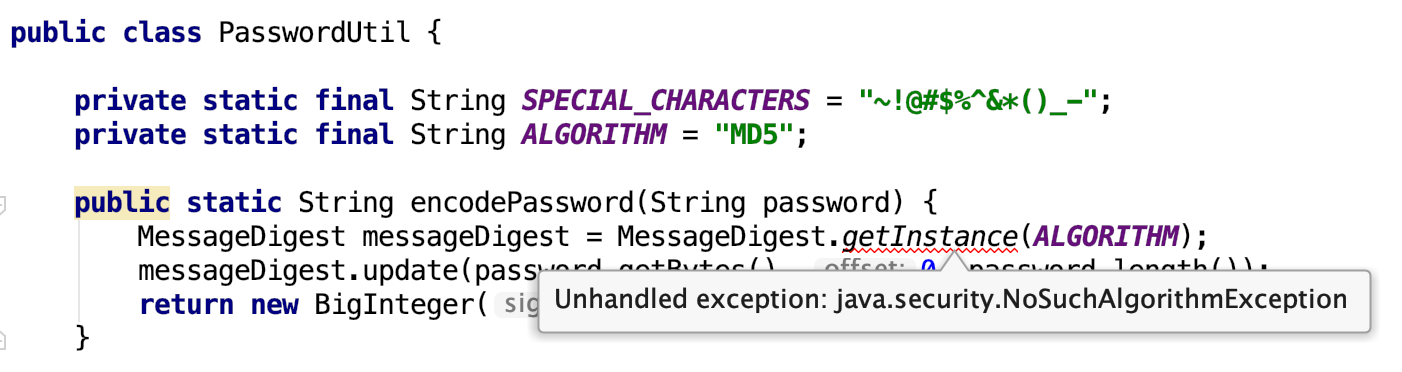
\includegraphics[width=\linewidth]{images/h2/no_such_algorithm_exception.png}
\caption{Een checked exception: NoSuchAlgorithmException}
\label{fig:no_such_algorithm}
\end{figure}

Deze compileerfout wordt veroorzaakt omdat de exception-klasse NoSuchAlgorithmException een checked exception is. Dit betekent dat het aanroepen van de methode die de exception gooit een compileerfout zal geven, omdat er geen code is toegevoegd om correct met de  exception om te gaan.
Er zijn 2 mogelijke oplossingen om deze compileerfout aan te pakken. Ofwel vang de exception op en handel je ze af in de methode calculateHash(), ofwel voeg je in de signatuur van de methode toe dat je de methode toelaat om een NoSuchAlgorithmException op te werpen. 

\begin{lstlisting}
package be.pxl.demo;

import org.slf4j.Logger;
import org.slf4j.LoggerFactory;
import org.springframework.stereotype.Service;

import java.security.MessageDigest;
import java.security.NoSuchAlgorithmException;

@Service
public class HashGeneratorService {

	private static final Logger LOGGER = LoggerFactory.getLogger(HashGeneratorService.class);

	public String calculateHash(String algorithm, String original) throws NoSuchAlgorithmException {
		MessageDigest md;
		md = MessageDigest.getInstance(algorithm);
		md.update(original.getBytes());
		byte[] digest = md.digest();
		StringBuilder result = new StringBuilder();
		for (byte b : digest) {
			result.append(String.format("%02x", b));
		}
		return result.toString();
	}
}
\end{lstlisting}

\begin{lstlisting}
package be.pxl.demo.api;

import be.pxl.demo.HashGeneratorService;
import be.pxl.demo.exception.InvalidMd5Exception;
import org.springframework.http.ResponseEntity;
import org.springframework.web.bind.annotation.GetMapping;
import org.springframework.web.bind.annotation.PathVariable;
import org.springframework.web.bind.annotation.PostMapping;
import org.springframework.web.bind.annotation.RequestBody;
import org.springframework.web.bind.annotation.RequestParam;
import org.springframework.web.bind.annotation.RestController;

import java.security.NoSuchAlgorithmException;

@RestController
public class MessageController {

	private final HashGeneratorService hashGeneratorService;

	public MessageController(HashGeneratorService hashGeneratorService) {
		this.hashGeneratorService = hashGeneratorService;
	}

	@GetMapping(value = "/hash/{algorithm}")
	public ResponseEntity<String> getHash(@PathVariable String algorithm, @RequestParam String text) {

		try {
			return ResponseEntity.ok(hashGeneratorService.calculateHash(algorithm, text));
		} catch (NoSuchAlgorithmException e) {
			return ResponseEntity.badRequest().build();
		}
	}
}

\end{lstlisting}

ResponseEntity is de representatie van het HTTP response: de statuscode, headers en body.  Je kan deze klasse gebruiken als je een andere statuscode wilt gegeven dan 200 (ok).

Hier is een overzicht van de meest voorkomende HTTP-statuscodes.

\begin{itemize}

\item \textbf{200 OK}: Dit is de standaard statuscode voor een succesvolle HTTP-aanvraag. Gebruik deze code om aan te geven dat de aanvraag met succes is verwerkt en dat de responsebody een antwoord bevat.  Deze statuscode wordt vaak gebruikt bij een succesvolle GET-request.

\item \textbf{201 Created}: Deze code geeft aan dat de aanvraag met succes is verwerkt en dat er een nieuwe resource is aangemaakt. Het wordt vaak gebruikt bij succesvolle POST-requests.

\item \textbf{204 No Content}: Deze statuscode geeft aan dat de aanvraag met succes is verwerkt, maar er is geen informatie is om terug te geven. Dit wordt vaak gebruikt voor succesvolle DELETE-aanvragen.

\item \textbf{400 Bad Request}: Gebruik deze code wanneer de client een ongeldige aanvraag heeft gedaan, bijvoorbeeld ontbrekende verplichte parameters of gegevens in een fout formaat.

\item \textbf{401 Unauthorized}: Dit geeft aan dat de client niet is geautoriseerd om toegang te krijgen tot de bron.  Meestal wordt dit gebruikt wanneer de client geen geldige authenticatiegegevens heeft verstrekt.

\item \textbf{403 Forbidden}: Hiermee geef je aan dat de client weliswaar is geauthenticeerd, maar geen toegang heeft tot de gevraagde bron vanwege beperkingen in de rechten of toegangsregels.

\item \textbf{404 Not Found}: Deze statuscode wordt gebruikt wanneer de gevraagde resources niet kan worden gevonden.

\item \textbf{500 Internal Server Error}: Dit geeft aan dat er een onverwachte fout is opgetreden aan de kant van de server. Het wordt vaak gebruikt voor fouten die niet direct kunnen worden toegeschreven aan de client.
\end{itemize}

\section{Multi-catch blok en finally}

\begin{lstlisting}
import java.util.Scanner;

public class MultiCatchBlockDemo {

	public static void main(String[] args) {
		Scanner scanner = new Scanner(System.in);
		System.out.println("Kies een positie: ");
		int positie = scanner.nextInt();
		System.out.println("Kies een deler: ");
		int deler = scanner.nextInt();
		try {
			int getallen[] = new int[10];
			getallen[positie] = 30 / deler;
		} catch (ArrayIndexOutOfBoundsException e) {
			System.out.println("Je moet een positie kiezen tussen 0 en 9.");
		} catch (Exception e) {
			System.out.println(e.getMessage());
		} finally {
			System.out.println("Je koos positie " + positie);
		}
		System.out.println("Start je het programma nog een keer.");
	}
}
\end{lstlisting}

Een try-blok kan gevolgd worden door \'e\'en of meerder catch-blokken.
Wanneer een exception optreedt zal bij het eerste catch-blok gestart worden. Indien onze exception een instantie is van de opgevangen exception  (instanceof) dan zal dat catch-blok uitgevoerd worden en worden de volgende catch-blokken niet meer bekeken. Indien de exception geen instantie is van de opgevangen exception dan wordt er verder gekeken naar de volgende catch-blokken tot een overeenkomstig catch-blok worden gevonden. Indien er geen catch-blok wordt gevonden zal de runtime-exception doorstromen naar de aanroepende methode.

De volgorde van de catch-blokken is van belang. ArrayIndexOutOfBoundsException is een subklasse van Exception. Als we eerst een catch-blok aanmaken voor de superklasse en pas daarna een catch-blok voor de subklasse zou het tweede catch-blok ``onbereikbaar'' zijn. Het eerste catch-blok gaat de exception reeds kunnen afhandelen. Code die onbereikbaar is (unreachable code) wordt opgemerkt door de compiler wat resulteert in een compileerfout van je code.

\begin{oefening}
Wissel beide catch-blokken eens van plaats in bovenstaande code.
\end{oefening}

Het finally-blok tenslotte is een codeblok dat altijd wordt uitgevoerd: of er nu een exception optreedt of niet. Zelfs als er een exception optreedt en die niet kan worden afgehandeld door een catch-blok, zal toch het finally-blok uitgevoerd worden.

\begin{oefening}
Test de werking van het finally-blok eens uit met bovenstaand programma MultiCatchBlockDemo. Verwijder het tweede catch-blok eens en veroorzaak een deling door 0. Wat gebeurt er?
\end{oefening}

Indien je dezelfde code hebt om verschillende exceptions af te handelen, mag je exceptions combineren in een catch-block. Zo zal het catch-blok in onderstaand voorbeeld zowel ArrayIndexOutOfBoundsExceptions als ArithmeticExceptions afhandelen.

\begin{lstlisting}
public class MultipleCatches {

	public static void main(String[] args) {
		Scanner scanner = new Scanner(System.in);
		System.out.println("Kies een positie: ");
		int positie = scanner.nextInt();
		System.out.println("Kies een deler: ");
		int deler = scanner.nextInt();
		try {
			int getallen[] = new int[10];
			getallen[positie] = 30 / deler;
		} catch (ArrayIndexOutOfBoundsException | ArithmeticException e) {
			System.out.println(e.getMessage());
		}
		System.out.println("Start je het programma nog een keer.");
	}
}
\end{lstlisting}

\section{Eigen unchecked exceptions}

We willen een endpoint toevoegen om te controleren of een MD5 hashcode correct is. 
Wanneer de berekende hashcode end de opgegeven hashcode niet overeenkomen gooien we een InvalidMd5Exception op.  Dit is een eigen unchecked exception. 

\begin{lstlisting}
package be.pxl.demo.exception;

public class InvalidMd5Exception extends RuntimeException {
	public InvalidMd5Exception() {
	}

	public InvalidMd5Exception(String message) {
		super(message);
	}

	public InvalidMd5Exception(String message, Throwable cause) {
		super(message, cause);
	}
}
\end{lstlisting}


\begin{lstlisting}
package be.pxl.demo;

import be.pxl.demo.exception.InvalidMd5Exception;
import org.slf4j.Logger;
import org.slf4j.LoggerFactory;
import org.springframework.stereotype.Service;

import java.security.MessageDigest;
import java.security.NoSuchAlgorithmException;

@Service
public class HashGeneratorService {

	private static final Logger LOGGER = LoggerFactory.getLogger(HashGeneratorService.class);

	public String calculateHash(String algorithm, String original) throws NoSuchAlgorithmException {
		MessageDigest md;
		md = MessageDigest.getInstance(algorithm);
		md.update(original.getBytes());
		byte[] digest = md.digest();
		StringBuilder result = new StringBuilder();
		for (byte b : digest) {
			result.append(String.format("%02x", b));
		}
		return result.toString();
	}

	public void verifyMd5(String original, String hash) {
		try {
			if (!calculateHash("MD5", original).equals(hash)) {
				throw new InvalidMd5Exception();
			}
		} catch (NoSuchAlgorithmException e) {
			LOGGER.error("Unexcepted exception", e);
			throw new InvalidMd5Exception("Invalid algorithm MD5",  e);
		}
	}
}
\end{lstlisting}

\begin{lstlisting}
package be.pxl.demo.api;

import be.pxl.demo.HashGeneratorService;
import be.pxl.demo.exception.InvalidMd5Exception;
import org.springframework.http.ResponseEntity;
import org.springframework.web.bind.annotation.GetMapping;
import org.springframework.web.bind.annotation.PathVariable;
import org.springframework.web.bind.annotation.PostMapping;
import org.springframework.web.bind.annotation.RequestBody;
import org.springframework.web.bind.annotation.RequestParam;
import org.springframework.web.bind.annotation.RestController;

import java.security.NoSuchAlgorithmException;

@RestController
public class MessageController {

	private final HashGeneratorService hashGeneratorService;

	@GetMapping(value = "/hash/{algorithm}")
	public ResponseEntity<String> hash(@PathVariable String algorithm, @RequestParam String text) {

		try {
			return ResponseEntity.ok(hashGeneratorService.calculateHash(algorithm, text));
		} catch (NoSuchAlgorithmException e) {
			return ResponseEntity.badRequest().build();
		}
	}

	@PostMapping(value = "/verify-md5")
	public ResponseEntity<Void> getMD5(@RequestBody RequestData data) {
		try {
			hashGeneratorService.verifyMd5(data.original(), data.md5());
			return ResponseEntity.noContent().build();
		} catch (InvalidMd5Exception e) {
			return ResponseEntity.status(418).build();
		}
	}
}
\end{lstlisting}